\section{Architecture}
This section describes the software architecture proposed by this project in order to realize the Transparent scheduling model over heterogeneous devices and, consequently, satisfy the requirements and use cases previously described.

\textit{Figure \ref{fig:architecture_complete}} provides a complete view of the Architecture; being a complex project based on the interaction between multiple distributed entities, the schema will be divided in three areas (easier to understand) that will be discussed in the following sections:
\begin{itemize}
    \item Cloud Services area (\textit{section \ref{cloud_services_area}})
    \item Contributor area (\textit{section \ref{contributor_area}})
    \item Customer area (\textit{section \ref{customer_area}})
\end{itemize}
\begin{figure}[!ht]
    \centering
    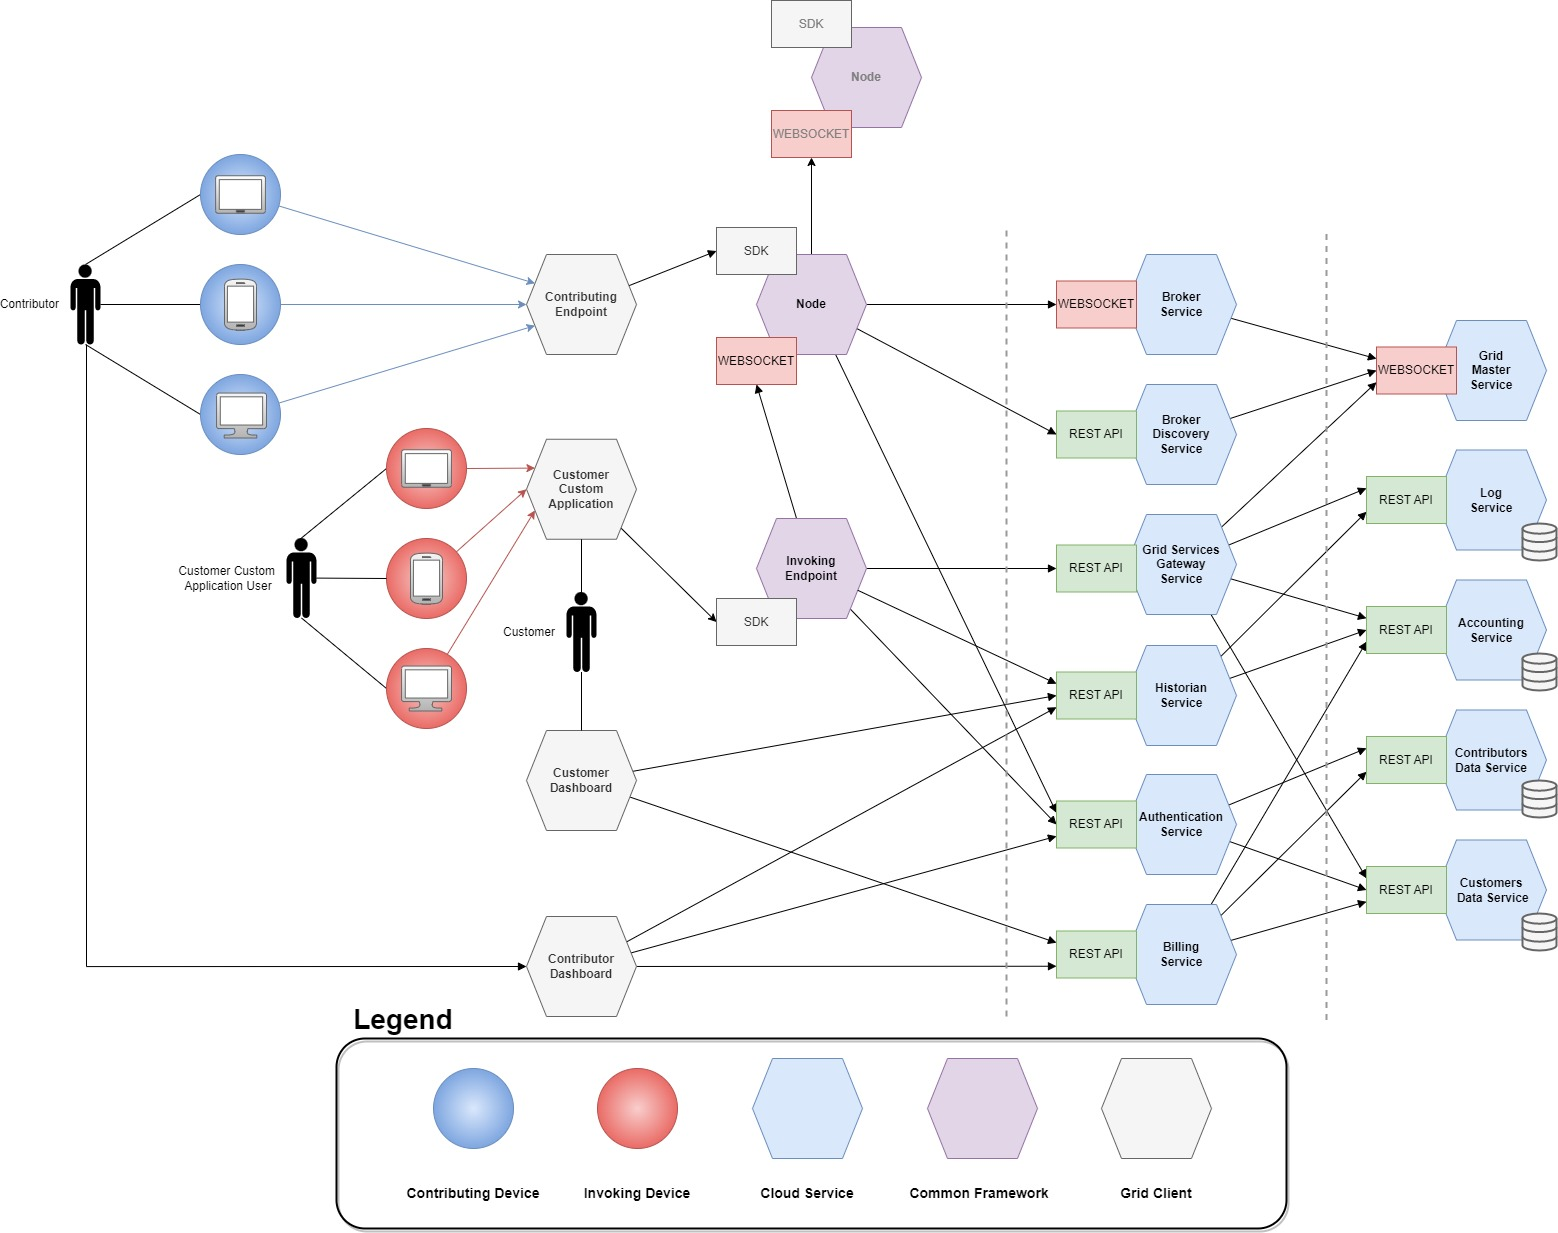
\includegraphics[width=\linewidth]{document/chapters/chapter_6/images/architecture_complete.jpg}
    \caption{Complete view of the Architecture}
    \label{fig:architecture_complete}
\end{figure}

\subsection{Cloud Services Area}\label{cloud_services_area}
The Cloud services follow a Hexagonal architecture composed by a multitude of microservices (\textit{Figure \ref{fig:architecture_cloud_services}}). Each Microservice is accessed through communication interfaces (whether Rest APIs or Web Sockets, depending on the particular microservice needs) and belong to one of the following layers:
\begin{itemize}
    \item \textbf{Business logic}\\
    Microservices that expose core business logic for Grid functionalities realization and data managing. Entities that  reside here are protected, meaning that they are isolated from the outside and their functionalities can only be accessed through the entities placed in the Adapters layer.
    \item \textbf{Adapters}\\
    Microservices that expose functionalities accessed by the entities residing in the Contributor and Customer area; such functionalities are realized through combining the services offered by entities residing in the Business logic layer.
\end{itemize}
\begin{figure}[!ht]
    \centering
    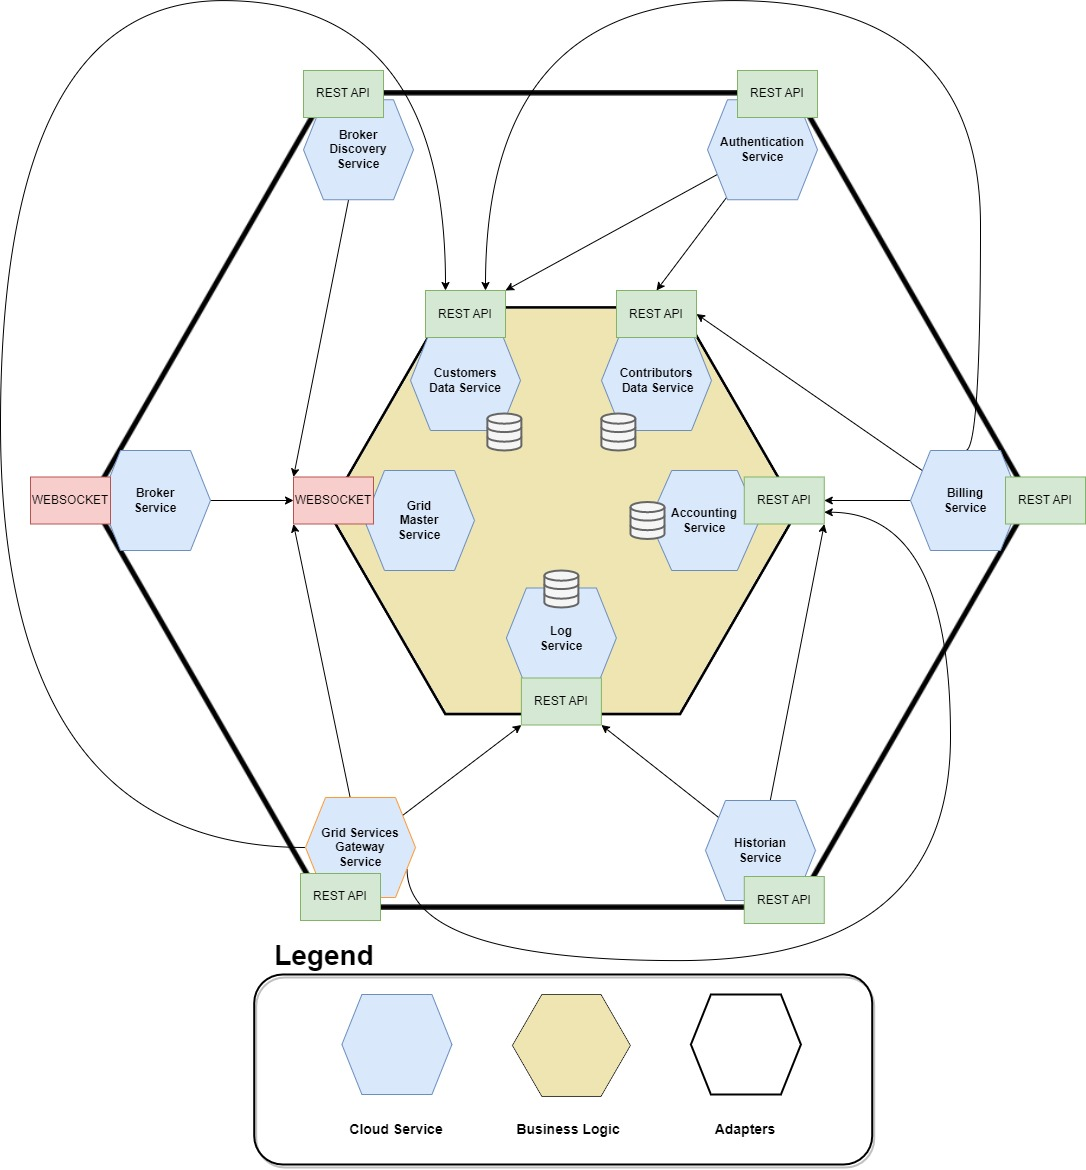
\includegraphics[scale=0.4]{document/chapters/chapter_6/images/architecture_cloud_services.jpg}
    \caption{Architecture: Cloud Services}
    \label{fig:architecture_cloud_services}
\end{figure}

\subsubsection{Business Logic}
\begin{itemize}
    \item \textbf{Grid Master Service}\\
    The main coordinator in the Grid system. It dynamically creates/removes Broker Service instances in order to sustain and balance the traffic generated by Nodes and Invoking Endpoints connected to the current instances of Broker Service; such instances needs to be contacted by Nodes but, being dynamically instantiated, they do not possess a static address. As a consequence of that, the Grid Master Service (that knows such addresses, being the creator of the instances) is connected to the Broker Discovery System (which will provide a Broker Service instance address to a connecting Node).

    \textit{Figure \ref{fig:master_grid_load_balancing}} shows a high level view of the connection between Grid Master, Brokers and Nodes while also providing an example of load balancing. When the new Node [N11] wants to connect to the Grid in order to Contribute, given that no Broker instance is able to handle the Node connection, the Grid Master instantiates [B2] to which [N11] will connect and part of the load handled by [B1] (just [N9] in this example) will be redirected to.
    \begin{figure}[!ht]
        \centering
        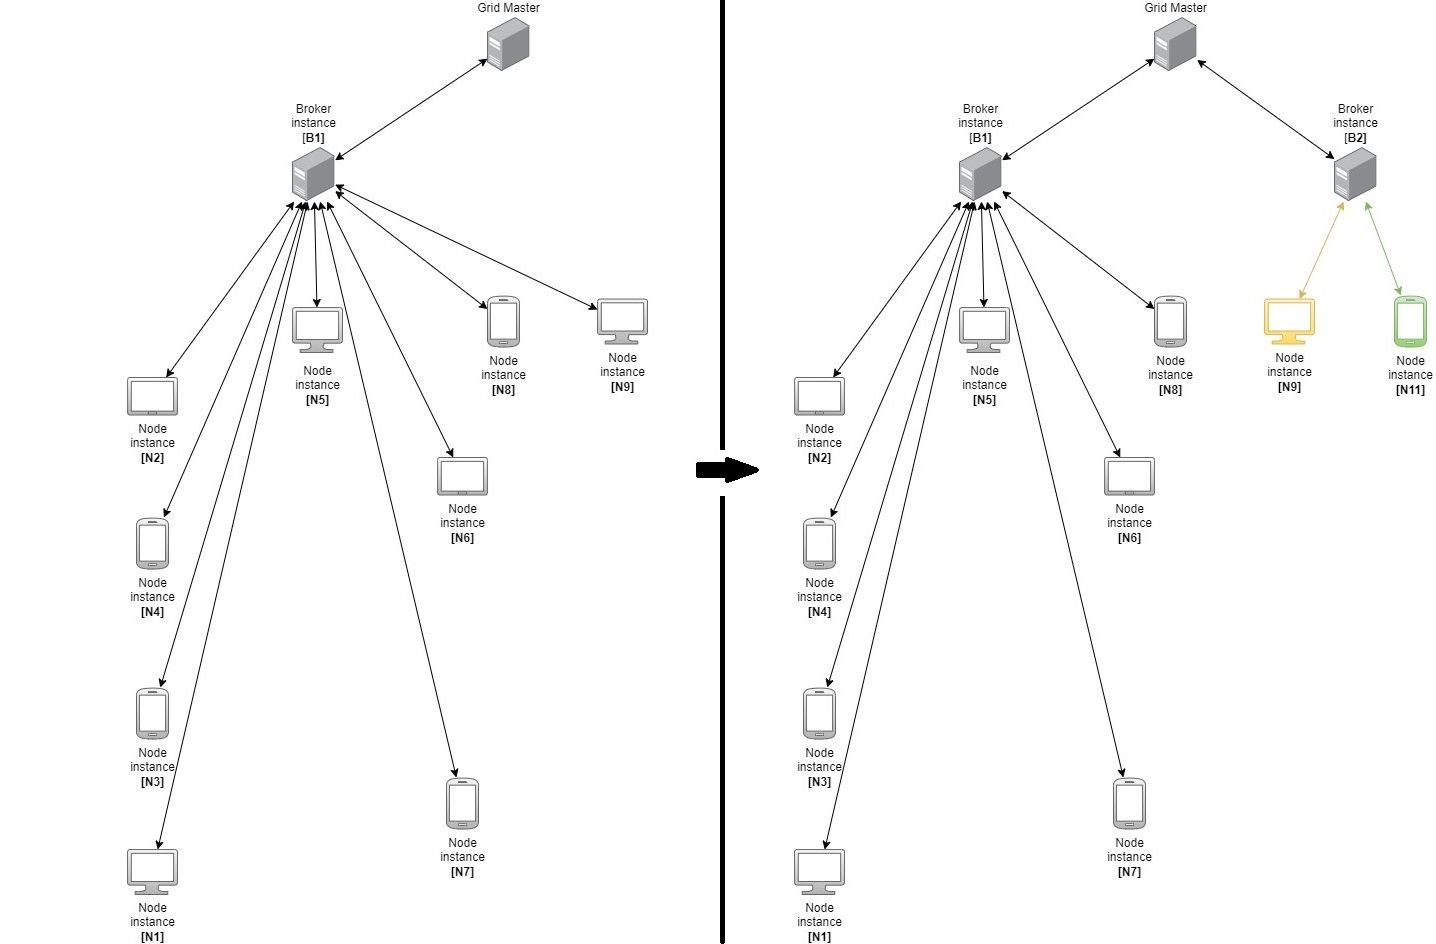
\includegraphics[width=\linewidth]{document/chapters/chapter_6/images/master_grid_load_balancing.jpg}
        \caption{Grid Master Service load balancing}
        \label{fig:master_grid_load_balancing}
    \end{figure}

    Lastly, the Grid Master Service is also connected to the Grid Services Gateway Service; through this last Cloud Service, the Invoking Endpoints request the execution of Grid Services. Thus, the Grid Master (collaborating with the Broker Service instances) will provide the Resources needed to execute the requested Grid Service.

    Concluding, this Cloud Service's importance is vital to the functioning and scalability of the Grid, requiring to expose communication interfaces for the discovery of Brokers, Resources obtainment and Grid coordination.

    \item \textbf{Customer Data Service}\\
    REST server that provides APIs used to read and write data used to uniquely identify a Customer inside the system. It does not contain data about payments or logs about Grid events that involve the Customer since those are handled by the Accounting Service and the Log Service respectively.\\
    Customers are, numerically speaking, considerably less compared to Contributors; this results in less frequent invocations of this Cloud Service's APIs and a far smaller volume of data to persist. Regarding the CAP theorem, it is then important to focus on a database technology that can grant Consistency and Partition Tolerance sacrificing Availability (e.g. MongoDB, BigTable, etc...).

    \item \textbf{Contributor Data Service}\\
    REST server that exposes APIs used to read and write data used to uniquely identify a Contributor and its devices inside the system. The same rules used in the Customer Data Service, regarding the handling of logs and payments data, also hold here; when it comes to the CAP theorem application, on the contrary, this Cloud Service requires AP database technologies (e.g. DynamoDB, Cassandra, etc...).

    \item \textbf{Accounting Service}\\
    TODO
    \item \textbf{Log Service}\\
    TODO
\end{itemize}

\subsubsection{Adapters}
TODO
\begin{itemize}
    \item \textbf{Broker Service}\\
    TODO
    \item \textbf{Broker Discovery Service}\\
    TODO
    \item \textbf{Grid Services Gateway Service}\\
    TODO
    \item \textbf{Authentication Service}\\
    TODO
    \item \textbf{Billing Service}\\
    TODO
    \item \textbf{Historian Service}\\
    TODO
\end{itemize}
\subsection{Contributor area}\label{contributor_area}
TODO

\begin{figure}[!ht]
    \centering
    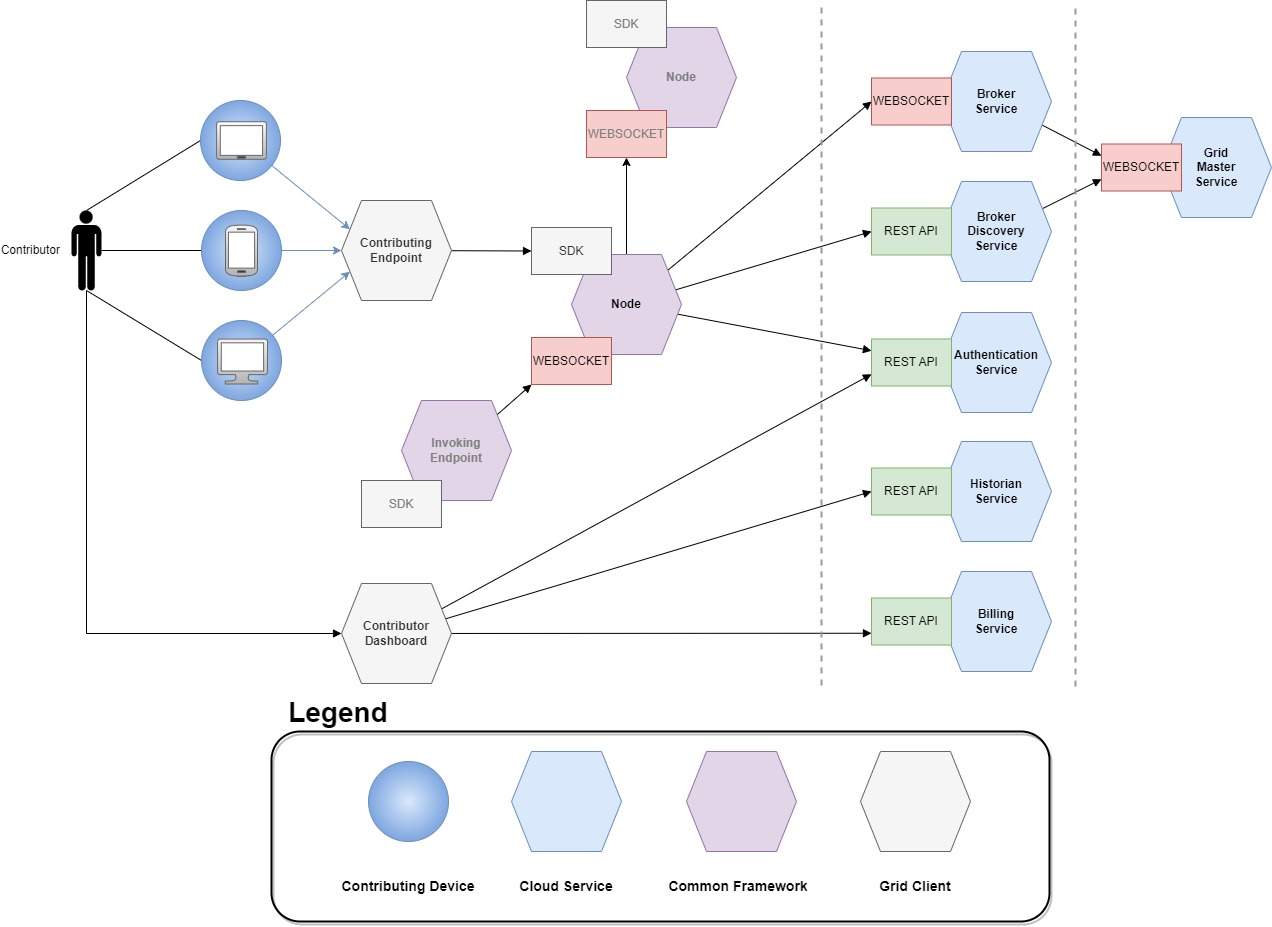
\includegraphics[width=\linewidth]{document/chapters/chapter_6/images/architecture_contributor.jpg}
    \caption{Architecture: Contributor-relevant view}
    \label{fig:architecture_contributor}
\end{figure}

\subsubsection{Node}
TODO
% High level grid draw.io: High level grid and Load Balancing

\subsubsection{Contributing Endpoint}
TODO
% Focus on interfaces and device-specific stuff

\subsubsection{Contributor Dashboard}
TODO
% Mockups

\subsection{Customer area}\label{customer_area}
TODO
\begin{figure}[!ht]
    \centering
    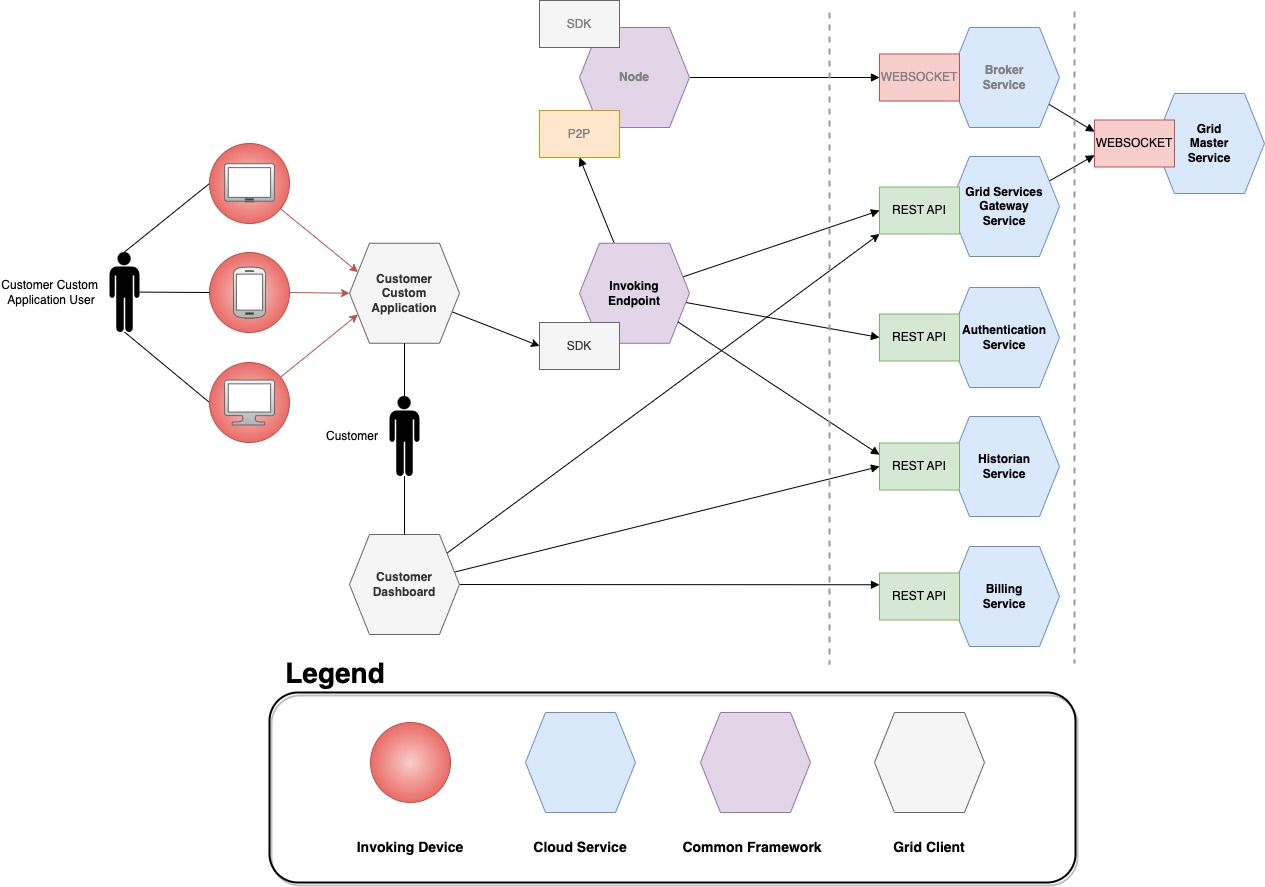
\includegraphics[width=\linewidth]{document/chapters/chapter_6/images/architecture_customer.jpg}
    \caption{Architecture: Customer-relevant view}
    \label{fig:architecture_customer}
\end{figure}

\subsubsection{Invoking Endpoint}
TODO
% High level grid draw.io: something similar to MapReduce but for a general task

\subsubsection{Customer Custom Application}
TODO
% focus on sdk

\subsubsection{Customer Dashboard}
TODO
% Mockups